\chapter{Entorno de desarrollo}

Este capítulo describe el proceso seguido para establecer el entorno de desarrollo, incluyendo los problemas que se encontraron, como se solucionaron y finalmente el resultado obtenido. Este entorno servirá de base para el trabajo posterior en los siguientes capítulos que, como está descrito en la sección de condiciones de diseño, tiene como función principal habilitar la validación del trabajo realizado por medio de la técnica ``Processor-in-Loop''.

\section{Selección de autopiloto base}

En el laboratorio de técnicas aeroespaciales se cuenta con hardware Pixhawk programado con el firmware de fábrica PX4. Existe un requisito que inmediatamente acota la selección de autopiloto, el software debe ser de código abierto debido a que posiblemente este se deba modificar en caso de que las prestaciones del software no sean suficientes para cumplir los objetivos.

\begin{figure}[h]
    \centering
    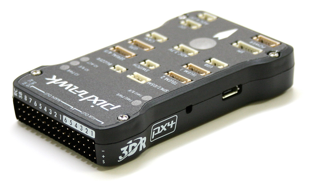
\includegraphics{hardware-pixhawk.png}
    \caption[Autopiloto Pixhawk.]{Autopiloto Pixhawk.\footnotemark}
    \label{fig:pixhawk1}
\end{figure}
\footnotetext{\url{https://docs.px4.io/v1.9.0/en/flight_controller/pixhawk.html}}

El hardware autopiloto Pixhawk se puede programar con otro software distinto al del fabricante, entre aquellas soluciones las que son aplicables según las condiciones de diseño y de código abierto son ArduPilot, iNAV y Paparazzi, además del mismo PX4 \cite{survey}. Revisando a un poco más detalle cada alternativa se puede notar que, iNAV no ofrece opciones de vuelo autónomo avanzadas como aterrizaje automático, que serán de interés en el capítulo de diseño de algoritmos de control. Paparazzi es una opción bastante interesante que si tiene un sistema autónomo completo por medio de archivos ``XML'' con la información del plan de vuelo \cite{paparazzi_flight_plan}, pero no es compatible con el software de control en tierra utilizado por ArduPilot y PX4, siendo Mission Planner y QGroundControl los principales.

\begin{figure}[h]
    \centering
    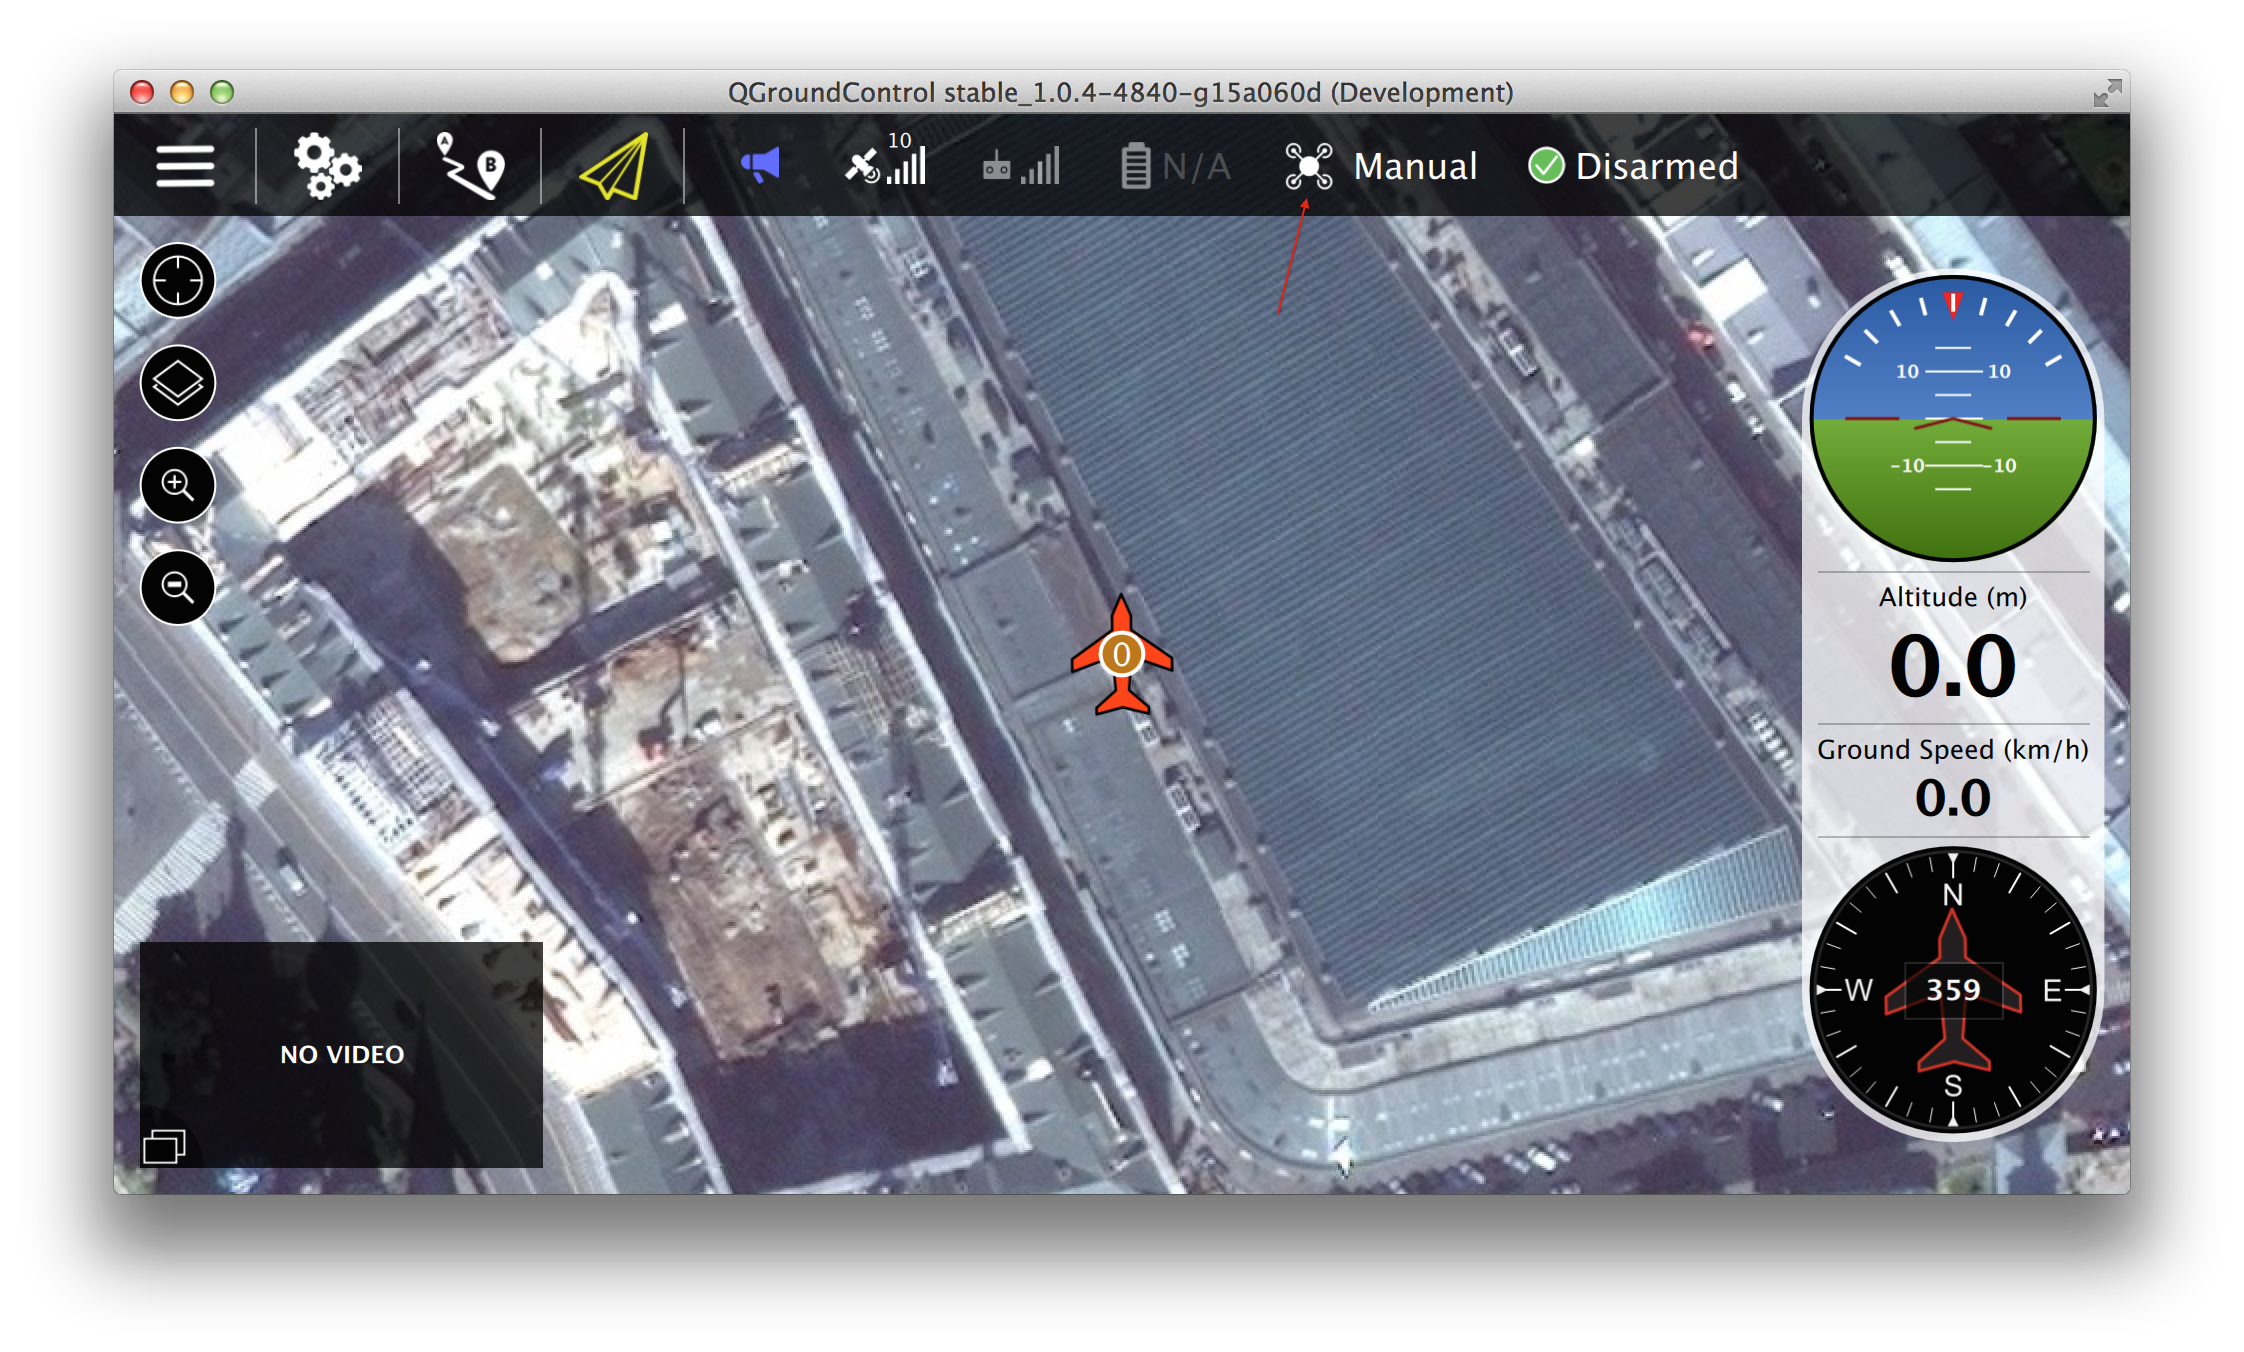
\includegraphics[width=0.7\textwidth]{qgroundcontrol.png}
    \caption[Software de estación en tierra QGroundControl.]{Software de estación en tierra QGroundControl.\footnotemark}
    \label{fig:qgroundcontrol}
\end{figure}
\footnotetext{\url{https://dev.px4.io/v1.11_noredirect/en/qgc/}}

PX4 es una opción atractiva ya que ofrece soporte para trabajar con técnicas ``Hardware-in-the-Loop'' con simuladores incluyendo X-Plane \cite{px4-hitl}. Sin embargo, aunque ArduPilot haya deprecado esa opción \cite{ap-hitl} existe más documentación en comparación con PX4 sobre como modificar existentes e implementar nuevos algoritmos de control \cite{ap-custom-controller}. Por esto último se decide en ArduPilot como plataforma de desarrollo.

\section{Extensión de protocolo de comunicación}

El protocolo de comunicación desarrollado durante el proyecto de ingeniería aeroespacial, inoFS, permite a X-Plane comunicarse con un microcontrolador. La interfaz disponible para lograrlo es aquella disponible en prácticamente todos los controladores, UART o mejor conocida como serial sobre USB. Para microcontroladores que ofrezcan acceso a la red por wifi o Ethernet inoFS también puede trabajar con paquetes UDP.

\begin{figure}[h]
    \centering
    \includesvg[width=0.7\textwidth]{diagrama-fssp.svg}
    \caption{Funcionamiento inoFS.}
    \label{fig:inofs-diagrama}
\end{figure}

Los detalles de su funcionamiento están en el informe de proyecto de ingeniería, pero cabe destacar el ``Programa intermediario'' en \cref{fig:inofs-diagrama} que es el principal responsable de traducir y reenviar los mensajes entre el simulador y el microcontrolador, se puede observar el programa funcionando junto a X-Plane en \cref{fig:inofs-programa-intermediario}.

\begin{figure}[h]
    \centering
    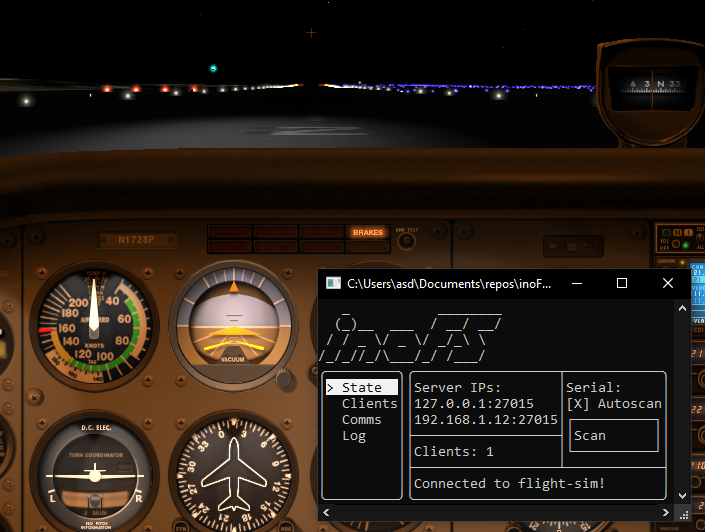
\includegraphics[width=0.6\textwidth]{inofs.png}
    \caption{Programa intermediario de inoFS.}
    \label{fig:inofs-programa-intermediario}
\end{figure}

Para poder extender el protocolo de comunicación se debe ser capaz de realizar dos funciones, ingresar a ArduPilot el estado de vuelo de X-Plane como respuesta obtenida de sensores, y el ejecutar las acciones de control producidas por ArduPilot en X-Plane. Con estas funciones se puede considerar lista la implementación ``Processor-in-Loop'' y a continuación se describe el proceso para lograr cada una.

\subsection{Ingresar información de sensores a ArduPilot}

La primera opción a evaluar para poder entregarle a ArduPilot información de sensores es la descrita en la metodología en el capítulo 1, emular la misma respuesta que producirían sensores de verdad con algún microcontrolador y comunicarla por los puertos apropiados como son los de \cref{fig:pixhawk-ports}. Para sensores sencillos que producen una respuesta análoga como un potenciómetro esto es posible, pero los sensores utilizados en RPAS en su mayoría son digitales, por ejemplo los sensores en el Pixhawk disponible en el laboratorio son los siguientes \cite{pixhawk1}.

\begin{itemize}
    \item ST Micro L3GD20H 16 bit gyroscope
    \item ST Micro LSM303D 14 bit accelerometer / magnetometer
    \item Invensense MPU 6000 3-axis accelerometer / gyroscope
    \item MEAS MS5611 barometer
\end{itemize}

Todos son sensores digitales, esto significa que al iniciar el sistema se les entrega alguna opción de configuración con la ayuda de un driver, y luego estos responden con las lecturas en un formato específico para cada sensor en forma de paquetes discretos. Por ejemplo el giroscopio L3GD20H espera que el microcontrolador (en este caso el que esté programado con ArduPilot) haga lecturas a ubicaciones en memoria del giroscopio \cite{gyro-datasheet}. Una de las ubicaciones de memoria en el giroscopio contiene información de sí las lecturas se han visto saturadas o si hay un valor nuevo como se ve en \cref{fig:gyro-health}. Emular cada sensor a una suficiente fidelidad capaz de ``engañar'' a ArduPilot de que está recibiendo lecturas reales es demasiado trabajo, por lo que se decide buscar alternativas.

\begin{figure}[h]
    \centering
    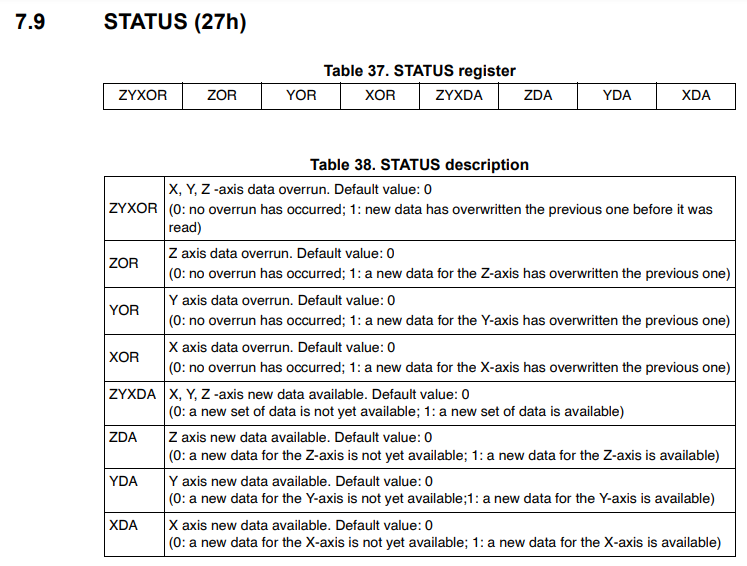
\includegraphics[width=0.6\textwidth]{gyro-registers.png}
    \caption{Ubicación en memoria del giroscopio con información de salud de las lecturas.}
    \label{fig:gyro-health}
\end{figure}

El hardware autopiloto donde puede funcionar ArduPilot (como es el Pixhawk disponible en el laboratorio) incluye puertos serial disponibles para muchas funciones como son el recibir lecturas de sensores que trabajen con esa interfaz, enviar y recibir mensajes que utilizan el protocolo de telemetría MavLink \cite{ap-serial} o para alguna aplicación personalizada que el usuario quisiera programar por medio de scripting en el lenguaje Lua \cite{ap-scripting}.

\begin{figure}[h]
    \centering
    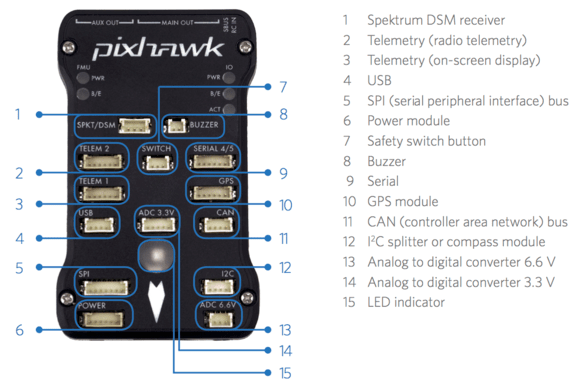
\includegraphics[width=0.6\textwidth]{pixhawk-ports.png}
    \caption[Puertos en Pixhawk.]{Puertos en Pixhawk.\footnotemark}
    \label{fig:pixhawk-ports}
\end{figure}
\footnotetext{\url{https://docs.px4.io/v1.9.0/en/flight_controller/pixhawk.html}}

La siguiente alternativa evaluada es enviar lecturas de sensores generadas con un protocolo propio por alguno de los puertos serial, y programar ArduPilot para que las interprete como lecturas de un sensor personalizado. Esto último es difícil, porque se debe programar, recompilar y cargar el nuevo firmware al autopiloto.

Primero se consideró aprovechar el motor de scripting en Lua para esta tarea. La ventaja de utilizar scripts es que no necesita modificar el código fuente de ArduPilot y por lo tanto tampoco reprogramar por completo el microcontrolador, ya que los scripts se cargan de manera dinámica desde la tarjeta SD. Lamentablemente los scripts no cuentan con la funcionalidad de poder generar lecturas de sensores críticos como son el IMU o GPS por lo que se descarta esta opción.

Estudiando el código fuente de ArduPilot se identificó que este soporta sistemas de estimación de actitud externos o ``External Attitude Heading Reference System'', están compuestos por una combinación de sensores y un procesador que realiza su propia fusión exportando un cuaternión describiendo la actitud junto con posición y velocidad en un marco de referencia inercial. Actualmente ArduPilot soporta tres sistemas de estimación de actitud externos disponibles en el mercado \cite{ap-eahrs}.

\begin{itemize}
    \item MicroStrain 3DM® Series
    \item VectorNav VN-300 AHRS
    \item VectorNav VN-100 AHRS
\end{itemize}

ArduPilot ofrece la opción de utilizar la estimación de actitud producida por el sistema externo directamente, o alternativamente solo recibir las mediciones de los sensores y por medio de un filtro de Kalman generar su propia estimación. En el contexto del proyecto ambas opciones son útiles, el que ArduPilot reciba la información de actitud perfecta de X-Plane permite descartar esta variable de los problemas que se vayan a producir durante las pruebas del controlador personalizado. Y el solo incorporar las lecturas de sensores y que ArduPilot realice su propia estimación con filtro de Kalman es lo que este haría en un vuelo real.

Se decidió escribir un driver para un nuevo sistema de estimación de actitud externo ficticio el cual recibirá lecturas de sensor y actitud por medio de conexión serial, que además entregara por esta misma conexión la respuesta de la acción de control que esté produciendo ArduPilot como salidas de servo. La creación de este nuevo driver en el lado de ArduPilot implica que se debe modificar el código fuente, en \cref{fig:eahrs} se pueden observar los archivos que componen los sistemas de estimación de actitud externos existentes. La interfaz principal \texttt{AP\_ExternalAHRS} y la implementación de los sistemas ``MicroStrain'' y ``VectorNav'', en los archivos \texttt{AP\_ExternalAHRS\_MicroStrain5} y \texttt{AP\_ExternalAHRS\_VectorNav}. El código fuente del nuevo driver se escribió en los archivos \texttt{AP\_ExternalAHRS\_HITL}, hasta este punto con la implementación más básica que lograse compilar y ser cargada en un autopiloto de pruebas.

\begin{figure}[h]
    \centering
    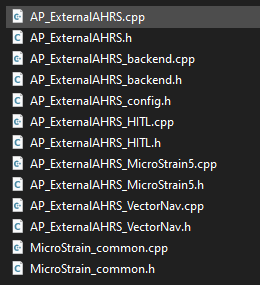
\includegraphics[width=0.3\textwidth]{eahrs.png}
    \caption{Archivos de código fuente para sistemas de estimación de actitud externos.}
    \label{fig:eahrs}
\end{figure}

El proceso de compilación de ArduPilot está documentado \cite{ap-build} y los firmware modificados se pueden cargar al autopiloto por USB de la misma forma que el oficial. En el laboratorio de técnicas aeroespaciales se proporcionó de un autopiloto Pixhawk 4 soportado por los desarrolladores de ArduPilot \cite{pixhawk4}. Para realizar la modificación del firmware de manera ordenada se creó un ``fork'' de la versión estable de ArduPlane en el momento de escritura del informe 4.4.2, sobre la que se escribe el nuevo driver y se lleva un registro de cada cambio en el repositorio en GitHub \cite{ap-hitl-fork}.

Una vez cargado ArduPilot modificado, con el programa de estación en tierra Mission Planner se ajusta el parámetro que indica que se utilizara un sistema inercial externo como se puede observar en \cref{fig:missionplanner-params}. Mission Planner no reconoce el nombre de la nueva opción correctamente mostrando un espacio en blanco, pero al seleccionarla y reiniciar el autopiloto se puede comprobar que se está ejecutando el nuevo driver observando el registro como se ve en \cref{fig:missionplanner-log}.

\begin{figure}[h]
    \centering
    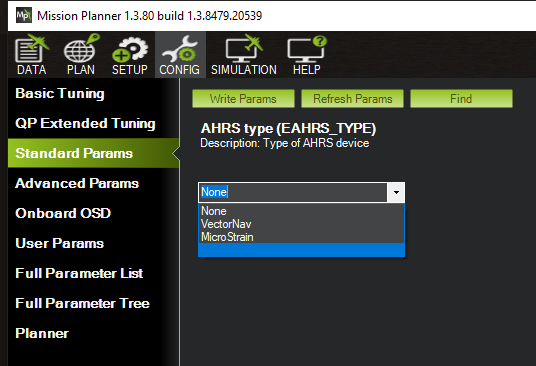
\includegraphics[width=0.6\textwidth]{missionplanner-params.png}
    \caption{Selección de sistema inercial externo en Mission Planner.}
    \label{fig:missionplanner-params}
\end{figure}

\begin{figure}[h]
    \centering
    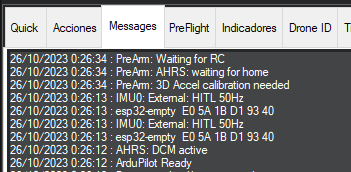
\includegraphics[width=0.4\textwidth]{missionplanner-log.png}
    \caption{Registro de inicialización de Mission Planner.}
    \label{fig:missionplanner-log}
\end{figure}

Durante las pruebas se descubrió un nuevo posible problema, como ha sido descrito hasta ahora se busca extender el protocolo de comunicación creado en el proyecto de ingeniería, inoFS. Sin embargo existe una limitación producto de su diseño. inoFS en sí extiende FSUIPC, el cual es un plug-in para Microsoft Flight Simulator que permite lectura y escritura arbitraria de variables internas del simulador, XPUIPC es una reimplementación del plug-in compatible con X-Plane que trabaja de la misma forma que FSUIPC. El problema es que la frecuencia a la que FSUIPC o XPUIPC pueden leer información de la simulación no está definida, y los sensores encontrados en los autopilotos pueden llegar a entregar lecturas a una frecuencia de hasta 1000 Hz como lo hace el MPU-6000. Además de la incerteza de la velocidad de FSUIPC está la latencia producto de tener que enviar la información a través del programa intermediario. Para asegurar la máxima frecuencia de datos posible se decidió no utilizar inoFS, y en su lugar crear un plug-in específico para X-Plane que envíe información por puerto serial directo luego de cada paso de la simulación, eliminando cualquier retraso posible en el canal de comunicación. Se lleva registro del desarrollo del plug-in en un repositorio en GitHub \cite{xplane-hitl-plugin} de la misma manera que para el ``fork'' de ArduPilot.

\begin{figure}[h]
    \centering
    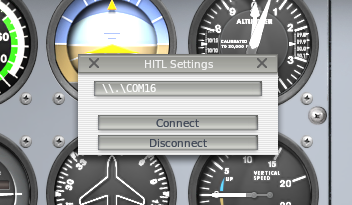
\includegraphics[width=0.4\textwidth]{hitl-plugin-1.png}
    \caption{Primera versión de plug-in ``HITL'' para X-Plane.}
    \label{fig:hitl-plugin-1}
\end{figure}

El desarrollo de plug-ins para X-Plane se realiza programando instrucciones en C++ y enlazando el SDK (Software Development Kit) que da acceso a una selección de librerías útiles para interactuar con el simulador \cite{xplane-plugin-dev}. El entorno de desarrollo en específico para este trabajo es Visual Studio Code con el compilador de Microsoft MSVC \cite{vscode-cpp}, los archivos disponibles en el repositorio incluyen la configuración (en el archivo \texttt{.vscode/tasks.json}) para poder compilar el plug-in en el editor de texto si se ha instalado MSVC.

El plug-in proporciona lecturas de sensor ficticio y la actitud de la aeronave por medio de la interfaz serial. En primera instancia el dispositivo serial seleccionado en el plug-in es un Raspberry Pi Pico conectado al computador por USB el cual retransmite la información al autopiloto también por serial por uno de los puertos de telemetría como se observa en \cref{fig:pi-pixhawk4,fig:plugin}. El programa cargado en el microcontrolador (utilizando el entorno de desarrollo Arduino IDE 2) solo realiza la tarea de retransmitir los datos recibidos por serial USB a serial por los pines GPIO 4 y 5 y el código para cumplir la función es \cref{lst:serial-passthrough}

\begin{listing}[h]
    \begin{minted}[frame=single,fontsize=\small]{C}
UART Serial2(4, 5, NC, NC);
void setup() {
    Serial.begin(115200);
    Serial2.begin(115200);
}
void loop() {
    if (Serial.available()) {
        Serial2.write(Serial.read());
    }
    if (Serial2.available()) {
        Serial.write(Serial2.read());
    }
}
    \end{minted}
    \caption{Retransmisor serial}
    \label{lst:serial-passthrough}
\end{listing}

\begin{figure}[h]
    \centering
    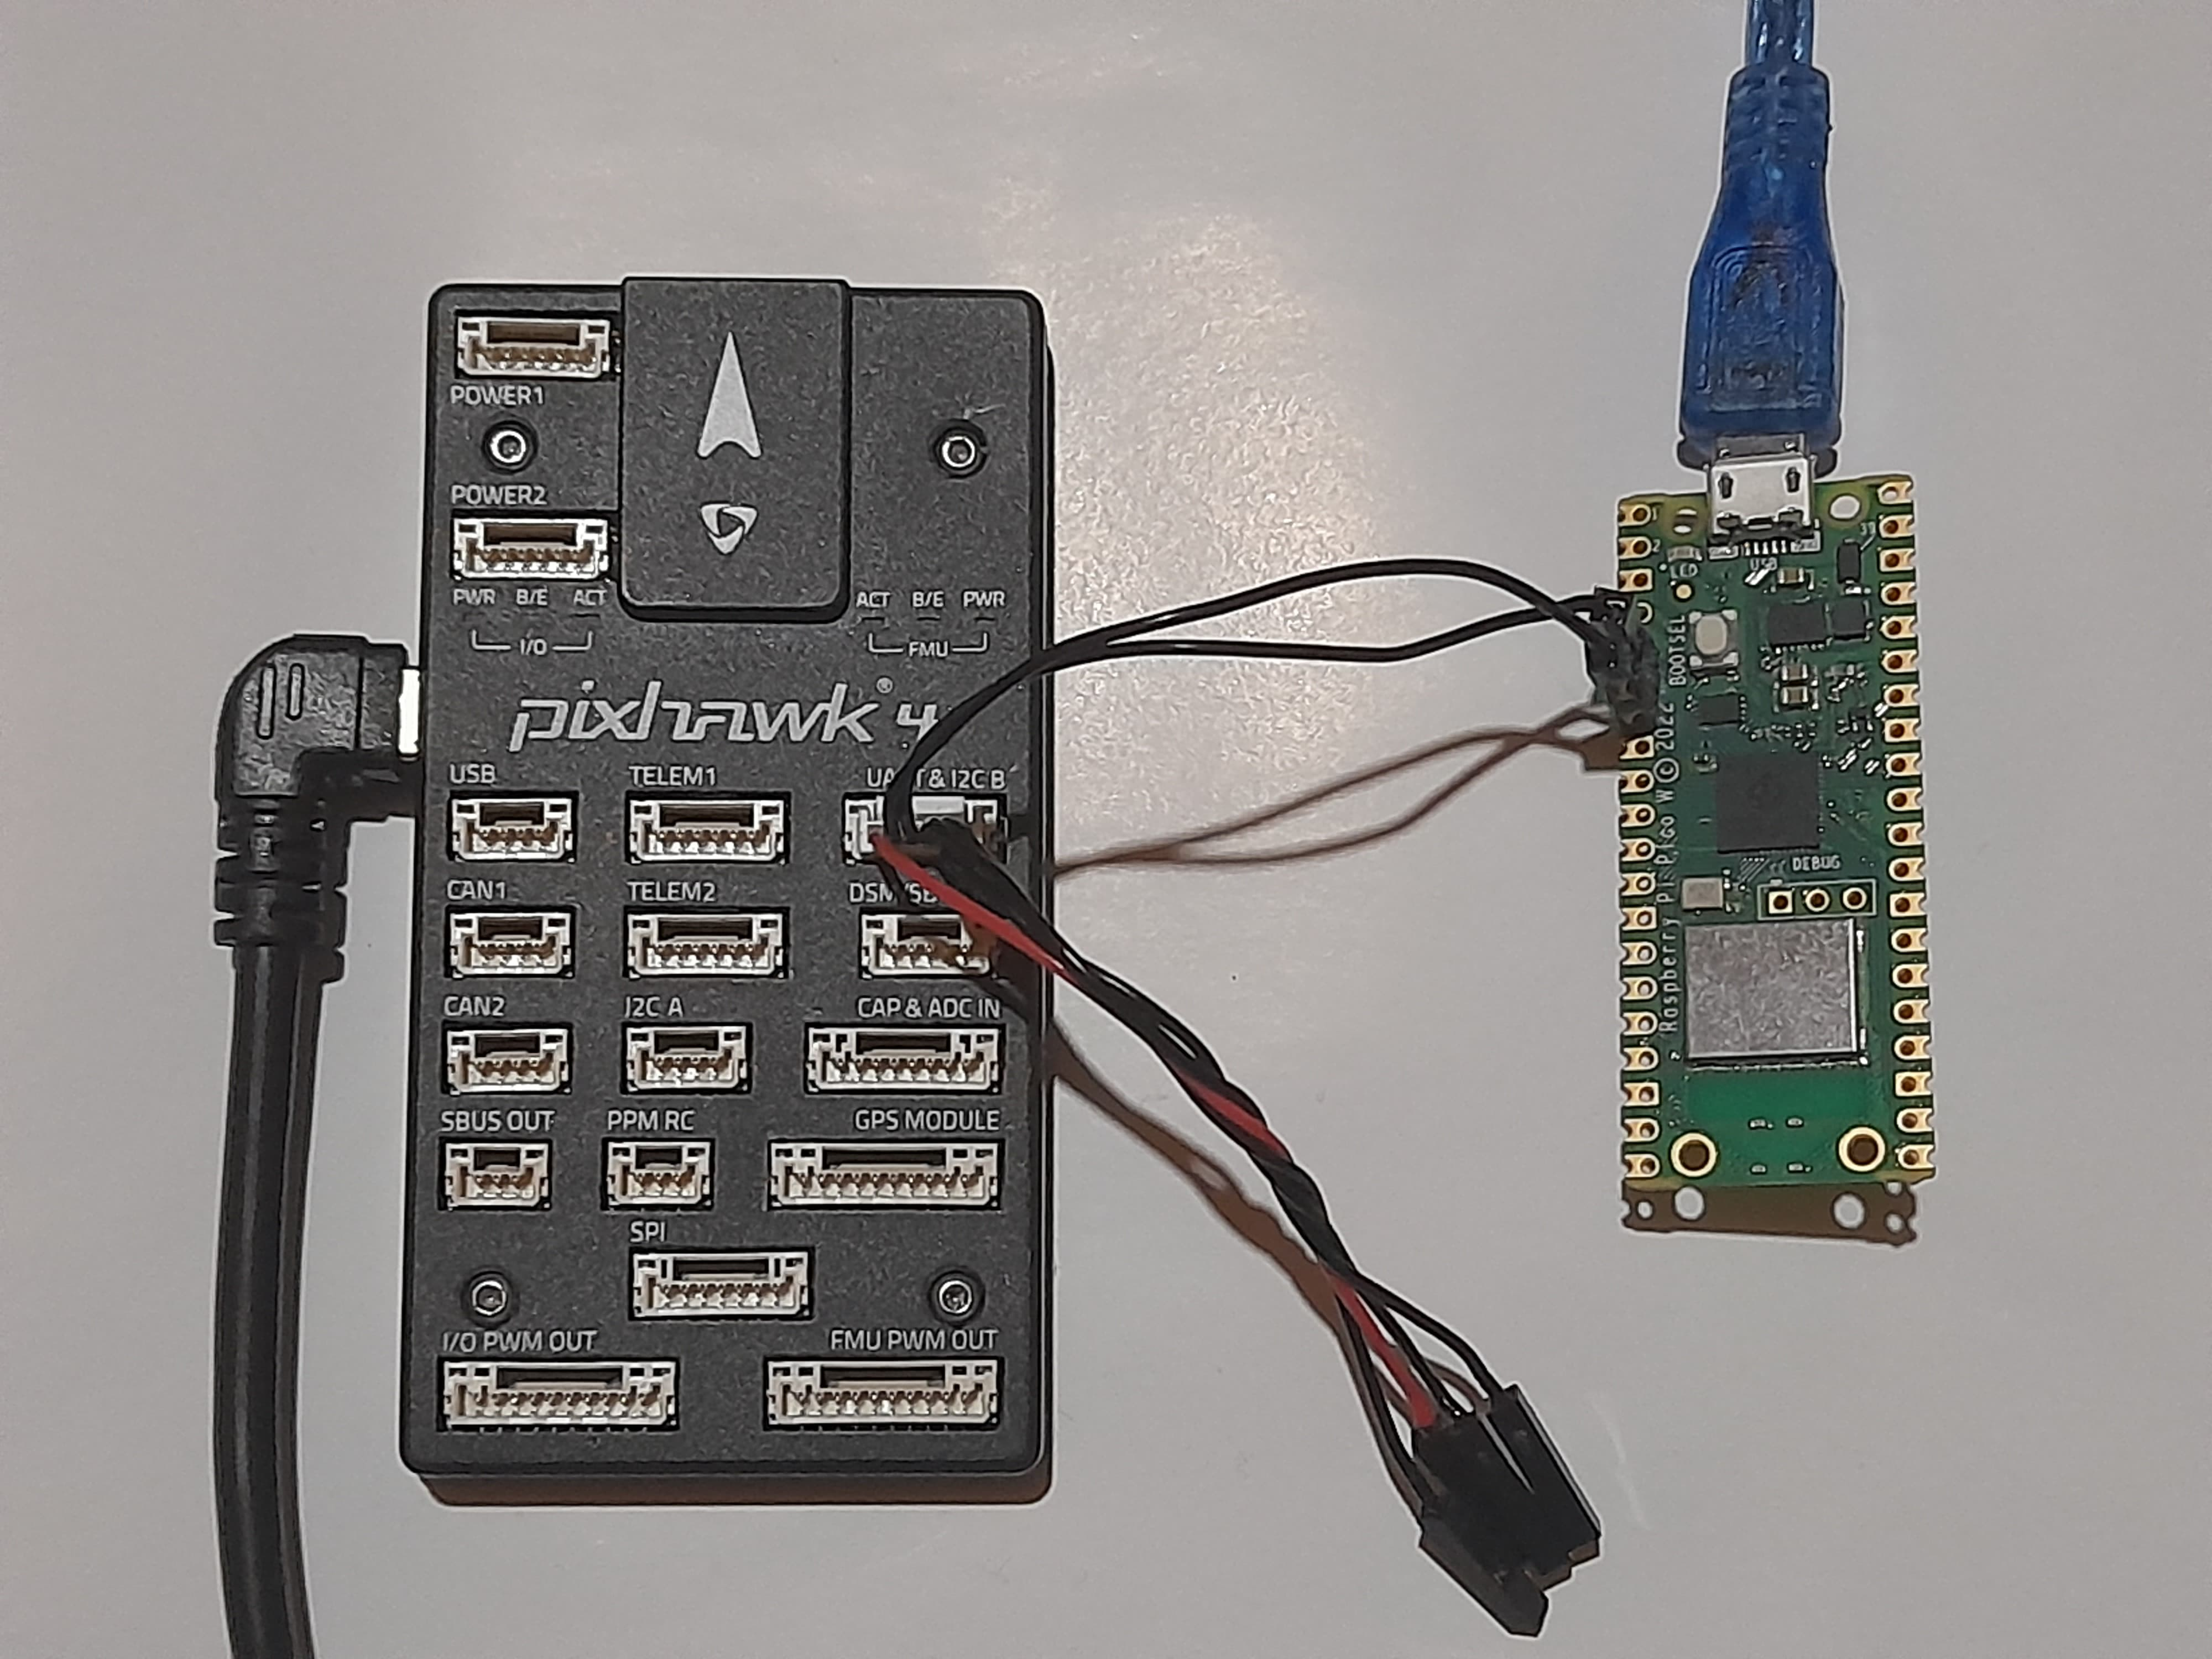
\includegraphics[width=0.5\textwidth]{pi-pixhawk4.jpeg}
    \caption{Raspberry Pi Pico conectado a Pixhawk 4.}
    \label{fig:pi-pixhawk4}
\end{figure}

\begin{figure}[h]
    \centering
    \includesvg[width=0.7\textwidth]{plugin.svg}
    \caption{Comunicación entre X-Plane y autopiloto.}
    \label{fig:plugin}
\end{figure}

Para terminar de conectar el Raspberry con el autopiloto, se configura el puerto de telemetría donde está conectado el microcontrolador como interfaz para sistema de estimación de actitud externo, como se observa en \cref{fig:missionplanner-params-serial} seleccionando la opción ``AHRS''.

\begin{figure}[h]
    \centering
    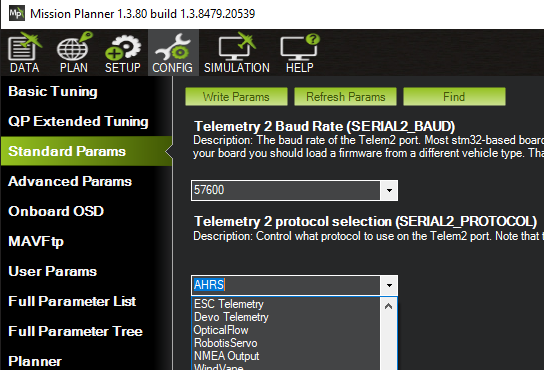
\includegraphics[width=0.6\textwidth]{missionplanner-params-serial.png}
    \caption{Especificación de función de puerto serial en Mission Planner.}
    \label{fig:missionplanner-params-serial}
\end{figure}

Con todo configurado se logra comprobar que la información de X-Plane está siendo procesada por el autopiloto, en \cref{fig:qgroundcontrol2} se observa que los movimientos del horizonte artificial del software en tierra (ahora QGroundControl) corresponden al de la inclinación de la aeronave. Hasta este punto se nota que el horizonte esta al revés porque aún falta procesar y calibrar un poco los datos para entregarlos en el formato que espera ArduPilot.

\begin{figure}[h]
    \centering
    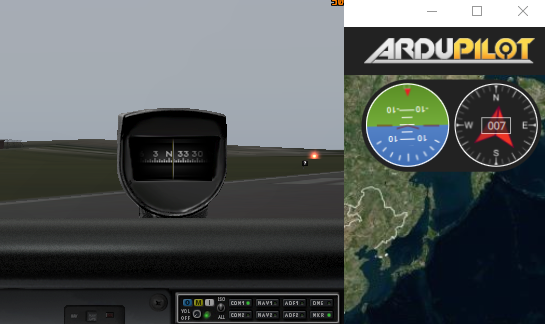
\includegraphics[width=0.6\textwidth]{xplane-qgroundcontrol.png}
    \caption{Lecturas de inclinación y orientación en QGroundControl.}
    \label{fig:qgroundcontrol2}
\end{figure}

Como mencionado anteriormente los sistemas de estimación de actitud externos ofrecen dos tipos de información, lecturas de sensores y estimación de la actitud exportada como un cuaternión. La manera en que ArduPilot espera recibir esta información está descrita en las estructuras de datos que se observan en \cref{lst:ap-structs-1,lst:ap-structs-2}.

\begin{listing}[h]
    \begin{minted}[frame=single,fontsize=\small]{C}
// Código de ArduPilot
// libraries/AP_ExternalAHRS/AP_ExternalAHRS.h
typedef struct {
    Vector3f accel;    // m/s2
    Vector3f gyro;     // rad/s 
    float temperature; // C
} ins_data_message_t;

typedef struct {
    uint8_t instance;
    float pressure_pa; // Pa
    float temperature; // C
} baro_data_message_t;

typedef struct {
    Vector3f field;
} mag_data_message_t;

typedef struct {
    uint16_t gps_week;
    uint32_t ms_tow;
    uint8_t fix_type;
    uint8_t satellites_in_view;
    float horizontal_pos_accuracy;
    float vertical_pos_accuracy;
    float horizontal_vel_accuracy;
    float hdop;
    float vdop;
    int32_t longitude;    // deg
    int32_t latitude;     // deg
    int32_t msl_altitude; // cm
    float ned_vel_north;  // m/s
    float ned_vel_east;   // m/s
    float ned_vel_down;   // m/s
} gps_data_message_t;
    \end{minted}
    \caption{Estructuras de datos para lecturas de sensor}
    \label{lst:ap-structs-1}
\end{listing}

Las estructuras de datos de lecturas de sensor corresponden a las de acelerómetro y giroscopio, barómetro, magnetómetro y GPS como aparecen respectivamente. Se debe obtener esta información de X-Plane por medio del plug-in y la forma en que este recopila los datos de la simulación es accediendo a los Dataref continuamente con la librería ``XPLMDataAccess'' del SDK \cite{xplane-dataref}, para la primera implementación del programa los Dataref utilizados se describen en \cref{lst:xplane-datarefs}. Los Dataref son variables internas de X-Plane que permiten acceder y modificar el estado de todos los componentes de la simulación, estos están disponibles de manera que desarrolladores pueden hacer uso fácilmente gracias a la extensa documentación \cite{xplane-dataref-ref}. La característica de enviar lecturas como telemetría por serial en el plug-in funciona en dos pasos, el primero es recopilar la información con los Dataref y el segundo es procesar los datos ya sea convertir unidades o generar la lectura del magnetómetro para luego enviarlos por serial como se observa en \cref{lst:telemetry-loop}, este proceso se repite en cada fotograma.

\begin{listing}[h]
    \begin{minted}[frame=single,fontsize=\small]{C}
// Código de plug-in para X-Plane
// telemetry.cpp
XPLMDataRef accel_x = XPLMFindDataRef("sim/flightmodel/forces/g_axil");
XPLMDataRef accel_y = XPLMFindDataRef("sim/flightmodel/forces/g_side");
XPLMDataRef accel_z = XPLMFindDataRef("sim/flightmodel/forces/g_nrml");
XPLMDataRef gyro_x = XPLMFindDataRef("sim/flightmodel/position/P");
XPLMDataRef gyro_y = XPLMFindDataRef("sim/flightmodel/position/Q");
XPLMDataRef gyro_z = XPLMFindDataRef("sim/flightmodel/position/R");
XPLMDataRef quat = XPLMFindDataRef("sim/flightmodel/position/q");
XPLMDataRef baro = XPLMFindDataRef("sim/weather/barometer_current_inhg");
XPLMDataRef temperature = XPLMFindDataRef("sim/weather/temperature_ambient_c");
XPLMDataRef latitude = XPLMFindDataRef("sim/flightmodel/position/latitude");
XPLMDataRef longitude = XPLMFindDataRef("sim/flightmodel/position/longitude");
XPLMDataRef elevation = XPLMFindDataRef("sim/flightmodel/position/elevation");
XPLMDataRef local_vx = XPLMFindDataRef("sim/flightmodel/position/local_vx");
XPLMDataRef local_vy = XPLMFindDataRef("sim/flightmodel/position/local_vy");
XPLMDataRef local_vz = XPLMFindDataRef("sim/flightmodel/position/local_vz");
    \end{minted}
    \caption{Datarefs utilizados para telemetría}
    \label{lst:xplane-datarefs}
\end{listing}

\begin{listing}[h]
    \begin{minted}[frame=single,fontsize=\small]{C}
// Código de plug-in para X-Plane
// telemetry.cpp
void Telemetry::Loop(float dt) {
    UpdateState();  // Recopilar información de Datarefs
    ProcessState(); // Procesar y enviar por serial
}
    \end{minted}
    \caption{Loop de telemetría en plug-in para X-Plane}
    \label{lst:telemetry-loop}
\end{listing}

La lectura del magnetómetro no se puede generar de manera realista utilizando solo las librerías en la SDK de X-Plane. Un magnetómetro entrega un vector que apunta al norte magnético de la tierra con magnitud proporcional a la ``intensidad'' del campo, el cual se puede describir en términos de la ``declinación'' e ``inclinación'' que son los ángulos que forma este vector respecto al norte geográfico como se observa en \cref{fig:magnetic-geographic-north}. X-Plane solo ofrece acceso a la declinación por medio del Dataref \texttt{sim\_flightmodel\_position\_magnetic\_variation}, no a la inclinación ni a la intensidad del campo. Sin embargo es posible obtener la inclinación e intensidad con librerías externas \cite{geomag}, puesto que el campo magnético de la tierra cambia muy lentamente. Durante el desarrollo del plug-in se realizaron pruebas entregando como lectura un vector que apunta perfectamente al norte geográfico y ArduPilot funciono correctamente. Hasta que no se retrabaje la implementación para hacerla más realista esta solución es suficiente.

\begin{figure}[h]
    \centering
    \includesvg[width=0.8\textwidth]{XYZ-DIS_magnetic_field_coordinates.svg}
    \caption[Diferencia entre norte magnético y geográfico.]{Diferencia entre norte magnético y geográfico.\footnotemark}
    \label{fig:magnetic-geographic-north}
\end{figure}
\footnotetext{\url{https://commons.wikimedia.org/wiki/File:XYZ-DIS_magnetic_field_coordinates.svg}}

Con ArduPilot recibiendo las lecturas de sensores de la manera esperada se logra observar correctamente el estado de la aeronave en Mission Planner, además el filtro de Kalman incluido en el autopiloto logra realizar la estimación de actitud exitosamente como se observa en \cref{fig:mission-planner-ok1}.

\begin{figure}[h]
    \centering
    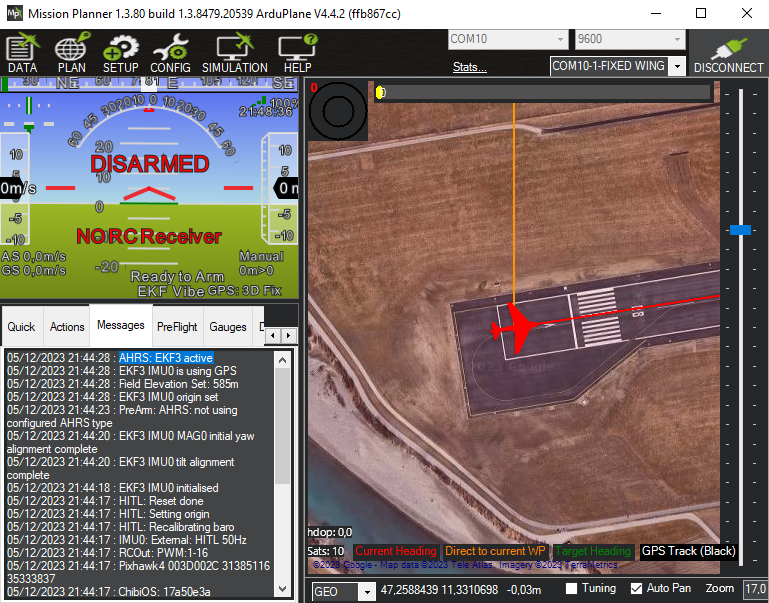
\includegraphics[width=0.9\textwidth]{mission-planner-ok1.png}
    \caption{Aeronave en Mission Planner.}
    \label{fig:mission-planner-ok1}
\end{figure}

La estructura de datos que describe la posición y actitud de la aeronave incluye varias de las mismas variables que se entregan como lecturas de sensor. Las excepciones son el cuaternión \texttt{quat} que describe la orientación y la posición \texttt{origin} que indica la posición inicial de la aeronave (antes de iniciar un despegue o una misión automatizada). La importante es el cuaternión el cual se obtiene directamente de X-Plane que de utilizarse permite omitir la necesidad de estimar la variable. Esta opción se puede activar modificando el parámetro \texttt{AHRS\_EKF\_TYPE} en Mission Planner como se ve en \cref{fig:missionplanner-params-ekf} seleccionando ``ExternalAHRS'', a diferencia de ``Enable EKF3'' que activa el filtro de Kalman del autopiloto recibiendo de X-Plane solo lecturas de sensor.

\begin{figure}[h]
    \centering
    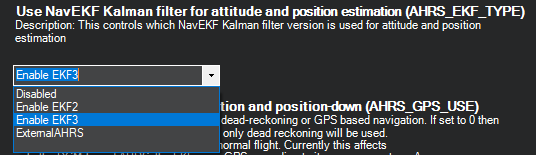
\includegraphics[width=0.7\textwidth]{missionplanner-params-ekf.png}
    \caption{Configuración de estimación de posición y actitud en Mission Planner.}
    \label{fig:missionplanner-params-ekf}
\end{figure}

\begin{listing}[h]
    \begin{minted}[frame=single,fontsize=\small]{C}
// Código de ArduPilot
// libraries/AP_ExternalAHRS/AP_ExternalAHRS.h
struct state_t {
    HAL_Semaphore sem;
    Vector3f accel;    // m/s2
    Vector3f gyro;     // rad/s
    Quaternion quat;
    Location location; // [hor: deg, deg, ver: cm]
    Vector3f velocity; // m/s  
    Location origin;   // [hor: deg, deg, ver: cm]
    bool have_quaternion;
    bool have_origin;
    bool have_location;
    bool have_velocity;
} state;
    \end{minted}
    \caption{Estructura de datos para posición y actitud}
    \label{lst:ap-structs-2}
\end{listing}

Si bien las lecturas de X-Plane llegan correctamente al autopiloto, estas no coinciden con las lecturas que producen los sensores internos del autopiloto. El Pixhawk 4 incluye acelerómetro, giroscopio, barómetro y magnetómetro los cuales son necesario desactivar para que no interfieran, el proceso para hacerlo se realiza por medio de modificación de parámetros en Mission Planner y configuración en una de las pestañas para el magnetómetro. A partir de una configuración por defecto de ArduPlane 4.4.2 los cambios a realizar son los siguientes.

\begin{enumerate}
    \item \textbf{Activar sistema de estimación de actitud externo.} \\
          Configurar los parámetros \texttt{EAHRS\_TYPE=3}, \texttt{SERIALX\_BAUD=115200} y \texttt{SERIALX\_PROTOCOL=36} de acuerdo al puerto serial correspondiente y reiniciar el autopiloto, asegurarse que en el registro aparezca habilitado el driver HITL.
    \item \textbf{Desactivar acelerómetro y giroscopio interno.} \\
          Configurar el parámetro \texttt{INS\_ENABLE\_MASK=1}.
    \item \textbf{Desactivar magnetómetro interno.} \\
          Configurar el parámetro \texttt{COMPASS\_TYPEMASK=252927}, desactivando todos los drivers excepto por el del sistema externo. Reiniciar el autopiloto e ir a la pestaña ``SETUP'' y en la sección ``Mandatory Hardware / Compass'' presionar ``Remove Missing'', reiniciar.
    \item \textbf{Activar GPS externo.} \\
          Configurar el parámetro \texttt{GPS\_TYPE=21}.
\end{enumerate}

\subsection{Ejecución de acciones de control en X-Plane}

Con la telemetría funcionando es posible habilitar las opciones de ArduPilot para ejecutar misiones automatizadas o las asistencias de estabilización de vuelo, siempre y cuando se tenga acceso a las superficies de control y potencia del motor. Las acciones de control de ArduPilot son exportadas como señales PWM de servo, para ArduPlane las salidas de servo por defecto son las superficies de control elevador, timón, alerón y el acelerador del motor \cite{arduplane-servo}. Internamente en el código fuente de ArduPilot los valores de salida se pueden obtener desde la clase \texttt{SRV\_Channels}, por lo que por medio de esta se realiza la lectura y posterior transmisión de información desde el autopiloto hacia X-Plane como se observa en \cref{lst:hitl-rc}.

\begin{listing}[h]
    \begin{minted}[frame=single,fontsize=\small]{C}
// Código de driver personalizado en ArduPilot
// libraries/AP_ExternalAHRS/AP_ExternalAHRS_HITL.cpp
void AP_ExternalAHRS_HITL::send_rc() {
    if (reset_step > 0) {
        rc_msg.state = reset_step + 1;
    } else {
        if (AP::arming().is_armed_and_safety_off()) {
            rc_msg.state = 1;
        } else {
            rc_msg.state = 0;
        }
    }
    rc_msg.aileron = SRV_Channels::get_output_norm(SRV_Channel::k_aileron);
    rc_msg.elevator = SRV_Channels::get_output_norm(SRV_Channel::k_elevator);
    rc_msg.rudder = SRV_Channels::get_output_norm(SRV_Channel::k_rudder);
    rc_msg.throttle = SRV_Channels::get_output_norm(SRV_Channel::k_throttle);
    rc_msg.ahrs_count = ahrs_count_send;
    uart->write(reinterpret_cast<uint8_t *>(&header), sizeof(header));
    uart->write(reinterpret_cast<uint8_t *>(&rc_msg), sizeof(rc_msg));
}
    \end{minted}
    \caption{Lectura y transmisión de salida de servos por serial}
    \label{lst:hitl-rc}
\end{listing}

Con los datos recibidos en el plug-in de X-Plane, se desactivan los controles convencionales del simulador que pueden ser el mouse o joysticks para las superficies de control y los motores. En su lugar se activa el control por medio de los Datarefs dedicados para esta aplicación como se observa en \cref{lst:xplane-plugin-rc}.

\begin{listing}[h]
    \begin{minted}[frame=single,fontsize=\small]{C}
// Código de plug-in para X-Plane
// remote.cpp
// ...
XPLMDataRef or_roll = XPLMFindDataRef("sim/operation/override/override_joystick_roll");
XPLMDataRef or_pitch = XPLMFindDataRef("sim/operation/override/override_joystick_pitch");
XPLMDataRef or_yaw = XPLMFindDataRef("sim/operation/override/override_joystick_heading");
XPLMDataRef or_throttle = XPLMFindDataRef("sim/operation/override/override_throttles");
XPLMDataRef roll = XPLMFindDataRef("sim/joystick/yoke_roll_ratio");
XPLMDataRef pitch = XPLMFindDataRef("sim/joystick/yoke_pitch_ratio");
XPLMDataRef yaw = XPLMFindDataRef("sim/joystick/yoke_heading_ratio");
XPLMDataRef throttle = XPLMFindDataRef("sim/flightmodel/engine/ENGN_thro_use");
// ...
if (override_joy) {
    XPLMSetDataf(DataRef::roll, std::clamp(servo_msg.aileron, -1.0f, 1.0f));
    XPLMSetDataf(DataRef::pitch, std::clamp(servo_msg.elevator, -1.0f, 1.0f));
    XPLMSetDataf(DataRef::yaw, std::clamp(servo_msg.rudder, -1.0f, 1.0f));
    float throttle[16];
    std::fill_n(throttle, 16, std::clamp(servo_msg.throttle, 0.0f, 1.0f));
    XPLMSetDatavf(DataRef::throttle, throttle, 0, 16);
}
// ...
    \end{minted}
    \caption{Datarefs para control de aeronave en plug-in de X-Plane}
    \label{lst:xplane-plugin-rc}
\end{listing}

Con estos cambios el autopiloto ya es capaz de controlar las superficies de control y el motor de la aeronave, sin embargo no es capaz de ``armar”, ya que aún se reportan problemas, estos son que se encuentran descalibrados el acelerómetro y magnetómetro entre otros como se observa en \cref{fig:arduplane-not-calibrated}. Para poder continuar es necesario calibrar estos sensores de la misma manera que se haría en una aeronave de verdad.

\begin{figure}[h]
    \centering
    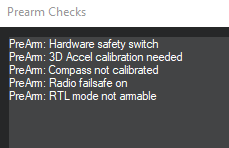
\includegraphics[width=0.35\textwidth]{arduplane-not-calibrated.png}
    \caption{Chequeos de prearmado.}
    \label{fig:arduplane-not-calibrated}
\end{figure}

\subsection{Calibración de acelerómetro y magnetómetro}

Antes de que ArduPilot permita armar la aeronave y así encender el motor es necesario realizar la calibración del acelerómetro y magnetómetro. El proceso consiste en ajustar la orientación de la aeronave paso a paso siguiendo las instrucciones en Mission Planner \cite{arduplane-accelerometer}.

Para el acelerómetro en la pestaña ``Accel Calibration'' se muestran instrucciones en pantalla como se observa en \cref{fig:ap-cal}. Se agregó la función de calibración en el plug-in para X-Plane que permite orientar la aeronave como se indica en Mission Planner, por medio de botones en la interfaz gráfica como se ve en \cref{fig:xplane-cal-level,fig:xplane-cal-left}.

\begin{figure}[h]
    \centering
    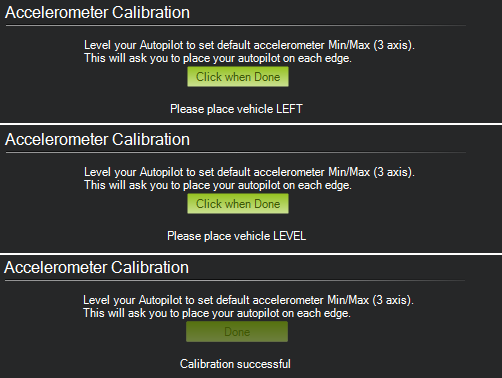
\includegraphics[width=0.52\textwidth]{ap-cal.png}
    \caption{Instrucciones de calibración de acelerómetro.}
    \label{fig:ap-cal}
\end{figure}

\begin{figure}[h]
    \centering
    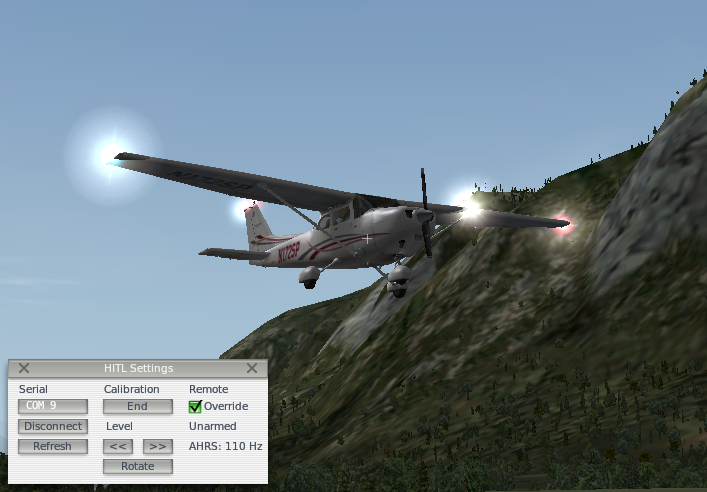
\includegraphics[width=0.7\textwidth]{xplane-cal-level.png}
    \caption{Aeronave en calibración nivelada.}
    \label{fig:xplane-cal-level}
\end{figure}

\begin{figure}[h]
    \centering
    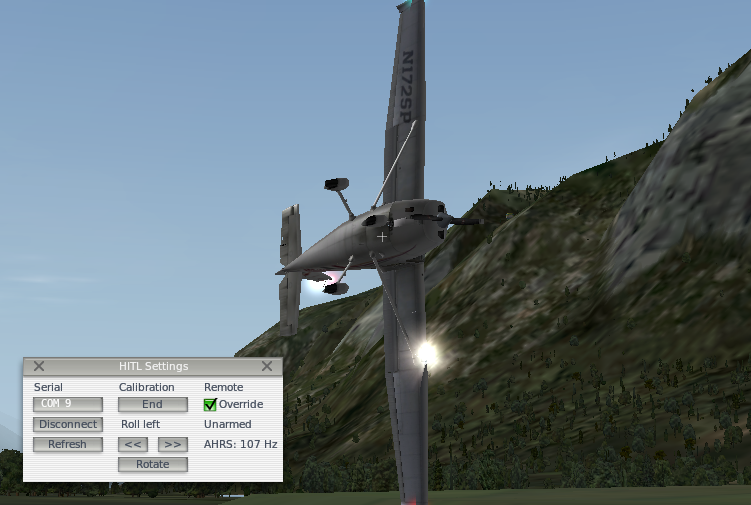
\includegraphics[width=0.7\textwidth]{xplane-cal-left.png}
    \caption{Aeronave en calibración inclinada a la izquierda.}
    \label{fig:xplane-cal-left}
\end{figure}

Elevar la aeronave y mantenerla quieta se logra sobreescribiendo todas las velocidades a 0, estableciendo posición y orientación específica y repetir ese proceso cada fotograma. Un problema que surge con este método es que la aceleración reportada por los Dataref es 0, siendo que debería ser un vector indicando la aceleración de gravedad. Se soluciona enviando por X-Plane el vector esperado, puesto que se conoce la orientación de la aeronave y la dirección que es hacia abajo en el marco de referencia inercial como está descrito en \cref{lst:accel-fix}.

\begin{listing}[h]
    \begin{minted}[frame=single,fontsize=\small]{C}
// Código de plug-in para X-Plane
// telemetry.cpp
// ...
// Inertial sensor
if (!Calibration::IsEnabled()) {
    msg.ins.accel = -state.accel * GRAVITY_MSS;
} else {
    Eigen::Vector3f down = { 0, 0, -GRAVITY_MSS };
    msg.ins.accel = state.rot.conjugate() * down;
}
// ...
    \end{minted}
    \caption{Vector de acelerómetro enviado por telemetría}
    \label{lst:accel-fix}
\end{listing}

La calibración del magnetómetro es similar, se debe orientar la aeronave de la misma manera que durante la calibración del acelerómetro, pero en cada paso se rota el rumbo una vuelta completa \cite{arduplane-compass}. El plug-in de X-Plane incluye un botón para empezar a rotar la aeronave de manera continua con este propósito como se observa en \cref{fig:xplane-cal-level,fig:xplane-cal-left}. De esta forma se logra calibrar el magnetómetro como se ve en \cref{fig:ap-cal-compass}.

\begin{figure}[h]
    \centering
    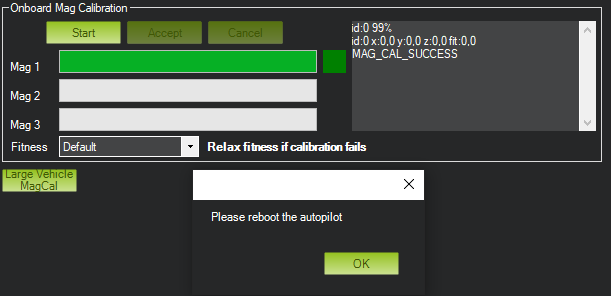
\includegraphics[width=0.7\textwidth]{ap-cal-compass.png}
    \caption{Calibración de magnetómetro completa en Mission Planner.}
    \label{fig:ap-cal-compass}
\end{figure}

Los otros problemas observados en los chequeos de prearmado en \cref{fig:arduplane-not-calibrated} reportan un ``Hardware safety switch'' y ``Radio failsafe on'', estos como su nombre indica son funciones de seguridad presentes en la aeronave y el radiocontrol. Para corregirlo se puede conectar un switch físico al autopiloto en el puerto correspondiente y activarlo, y en la radio desactivar la seguridad de acuerdo a las instrucciones de ArduPilot y la radio especifica. Otra forma es establecer los parámetros \texttt{BRD\_SAFETY\_DEFLT=0} para desactivar el safety switch y \texttt{THR\_FAILSAFE=0} para desactivar la seguridad de la radio. Con todo resuelto es posible armar la aeronave y utilizar Mission Planner tal cual se tratase de una aeronave real.

\subsection{Pruebas en X-Plane}

Conectando un receptor de radio al puerto correspondiente en el Pixhawk 4 se prueban distintas aeronaves en el simulador X-Plane 9 como se observa en \cref{fig:setup}. Entre las aeronaves disponibles por defecto se encuentran el Cessna 172 y un aeromodelo RC los cuales se logran volar de manera satisfactoria en los modos de vuelo estabilizado y en misión autónoma definida por waypoints en Mission Planner como se muestra en \cref{fig:xplane-rc}, incluso sin ajustar ningún parámetro del controlador PID.

\begin{figure}[h]
    \centering
    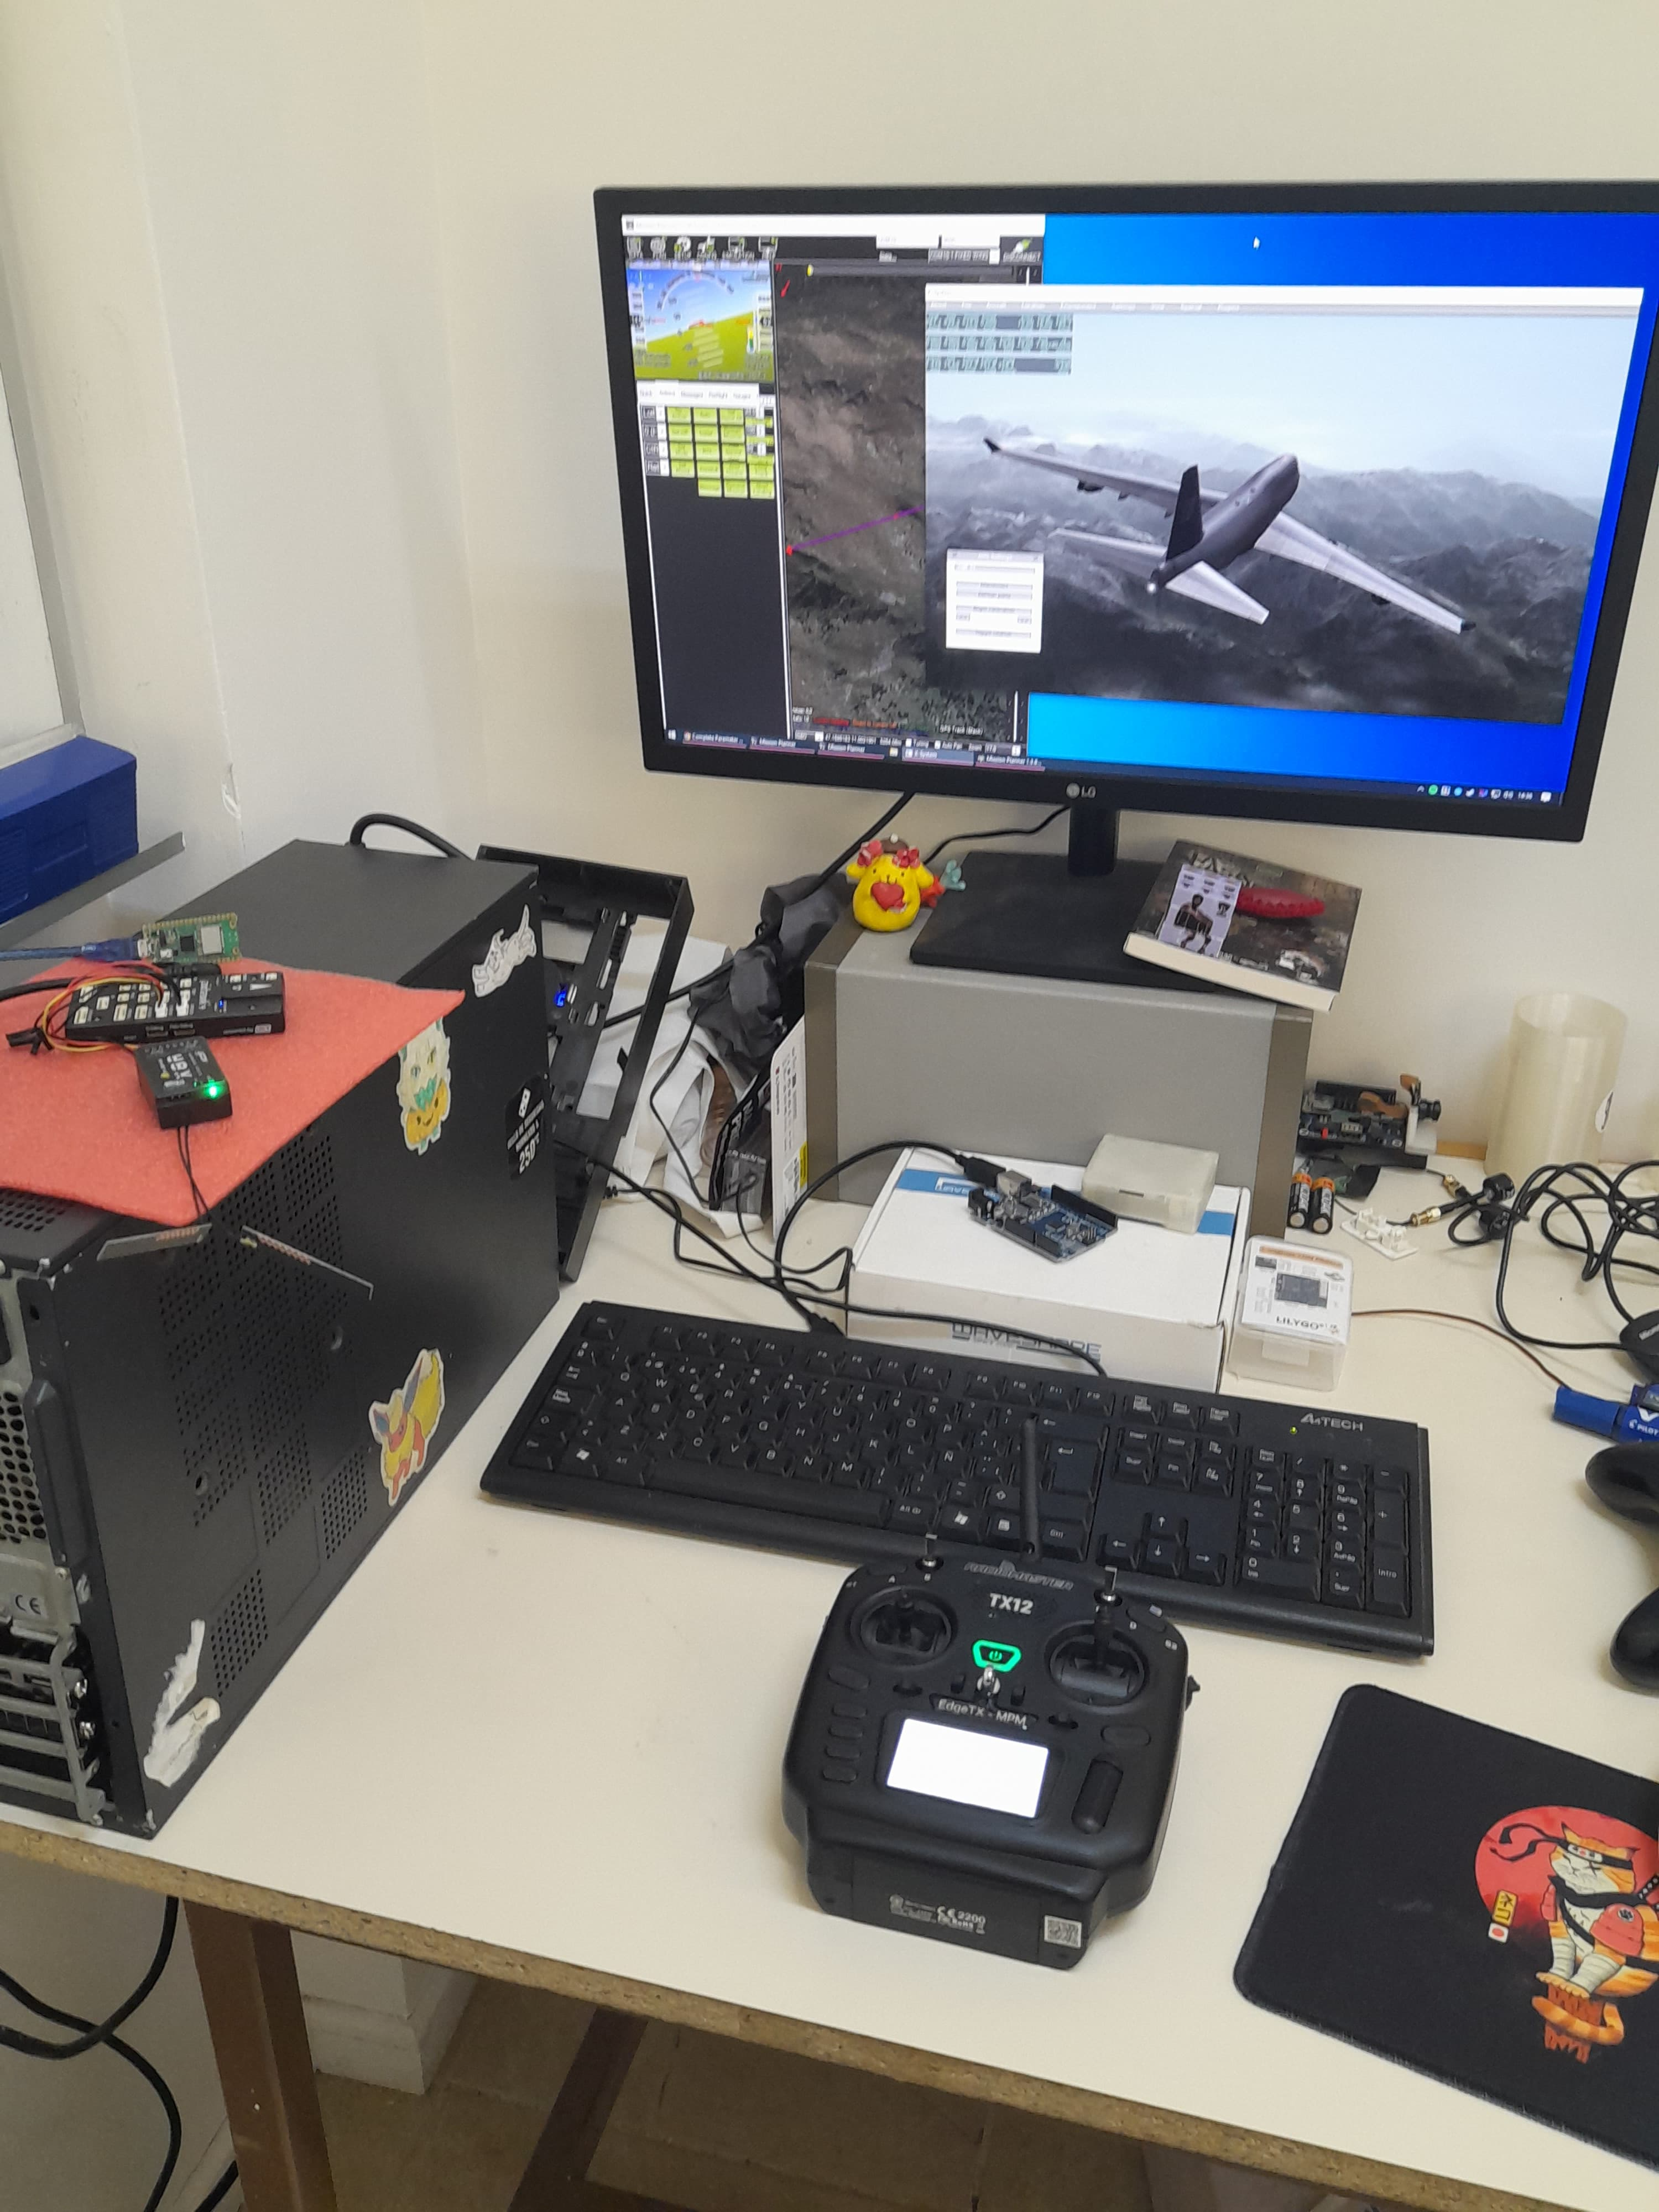
\includegraphics[width=0.4\textwidth]{setup.jpeg}
    \caption{Vuelo con radio en X-Plane 9.}
    \label{fig:setup}
\end{figure}

\begin{figure}[h]
    \centering
    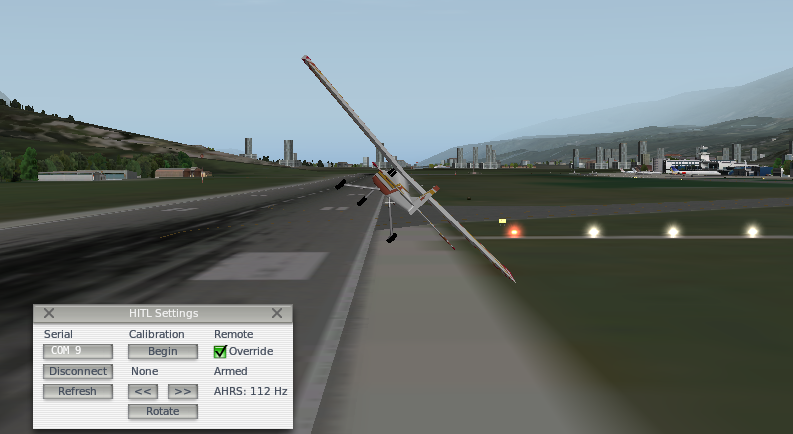
\includegraphics[width=0.6\textwidth]{xplane-rc.png}
    \caption{Aeronave RC en misión autónoma en X-Plane 9.}
    \label{fig:xplane-rc}
\end{figure}

En su estado actual el plug-in junto con el firmware modificado tienen potencial de ser utilizados para el aprendizaje del uso general de ArduPilot y Mission Planner, más en comparación con las soluciones SITL porque esta alternativa permite conectar un receptor RC real y realizar un proceso de calibración que emula el real. La continuación de su desarrollo para este propósito consiste en simular los defectos presentes en los sensores en lugar de transmitir lecturas perfectas.

Otra prueba fue compilar el plug-in para versiones más actualizadas de X-Plane como X-Plane 11. El plug-in funciona correctamente en esta versión del simulador abriendo las mismas posibilidades que con X-Plane 9.

\begin{figure}[h]
    \centering
    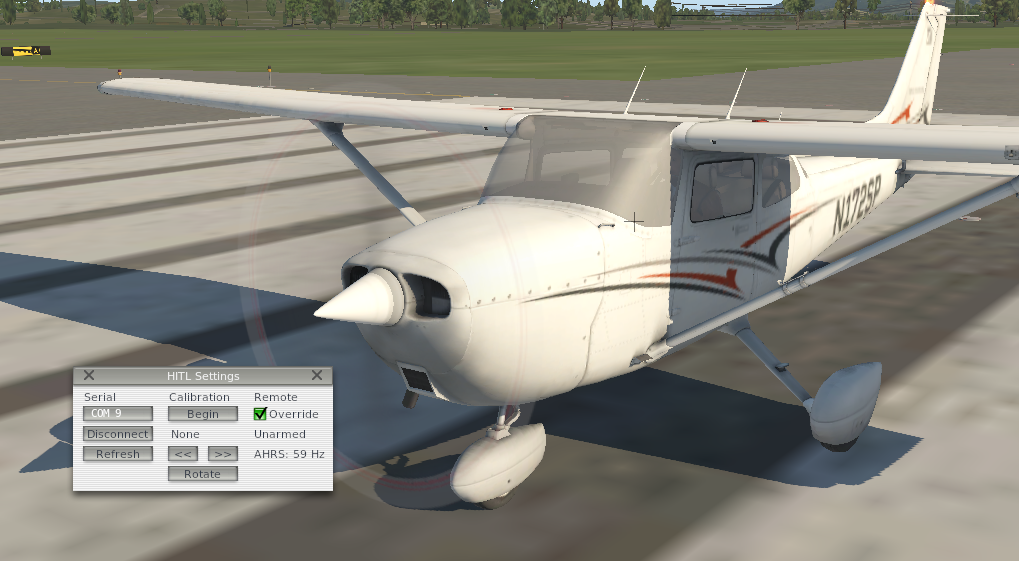
\includegraphics[width=0.8\textwidth]{xplane11.png}
    \caption{Plug-in funcionando en X-Plane 11.}
    \label{fig:xplane11}
\end{figure}

\subsection{Otros descubrimientos y problemas durante el desarrollo}

\textbf{Eliminación del microcontrolador intermediario}

Durante el desarrollo se descubrió que el autopiloto Pixhawk 4 abre dos puertos serial por la misma conexión USB, el primer puerto es el que se ha estado utilizando para conectarse por Mission Planner, el segundo se puede configurar para cualquier uso por medio de los parámetros y en Pixhawk 4 corresponde al puerto serial 7, si se configura este puerto como sistema de estimación de actitud externo el plug-in es capaz de conectarse y enviar información. Esto elimina la necesidad del Raspberry retransmisor lo cual es bastante conveniente.

\textbf{Problemas al teletransportar la aeronave}

Al seleccionar un nuevo aeropuerto, cambiar la aeronave o luego de un choque fatal X-Plane regenera la aeronave en la pista de aterrizaje independiente de donde se haya encontrado previamente. Este cambio brusco en la posición y orientación confunde al autopiloto el que comienza a reportar errores en la estimación de actitud entre otros. La solución encontrada fue reiniciar internamente las variables del filtro de Kalman integrado en el autopiloto luego de cualquier teletransporte. Realizar esto no es tan fácil, puesto que el autopiloto no incluye una función para hacerlo ni es una situación que ocurriría en la vida real. Reiniciar de manera arbitraria el filtro de Kalman a veces detenía por completo el autopiloto el cual reportaba errores internos críticos luego de ser encendido la próxima vez. Corregir esto fue un proceso de prueba de error restableciendo las variables internas una por una hasta lograr una secuencia que no detuviera el autopiloto, pero que reinicia el filtro.

\subsection{Puesta en marcha}

La primera versión del entorno de desarrollo compuesto por el plug-in y driver cumple para continuar pruebas de modificaciones posteriores que se hagan en ArduPilot y también promete ser una gran herramienta de aprendizaje en el funcionamiento de un autopiloto y el uso de Mission Planner. Poner en marcha el entorno en un computador que no sea el de desarrollo consiste en descargar el plug-in para X-Plane desde el repositorio en GitHub \cite{xplane-hitl-plugin} y descargar el firmware del autopiloto que se tenga disponible también en el repositorio correspondiente \cite{ap-hitl-fork} para programarlo con Mission Planner. Se han subido a ambos repositorios las instrucciones básicas para configurar el entorno de desarrollo como se observa en \cref{fig:repo-ap,fig:repo-plugin}, equivalentes a los pasos descritos durante el desarrollo del capítulo.

\begin{figure}[h]
    \centering
    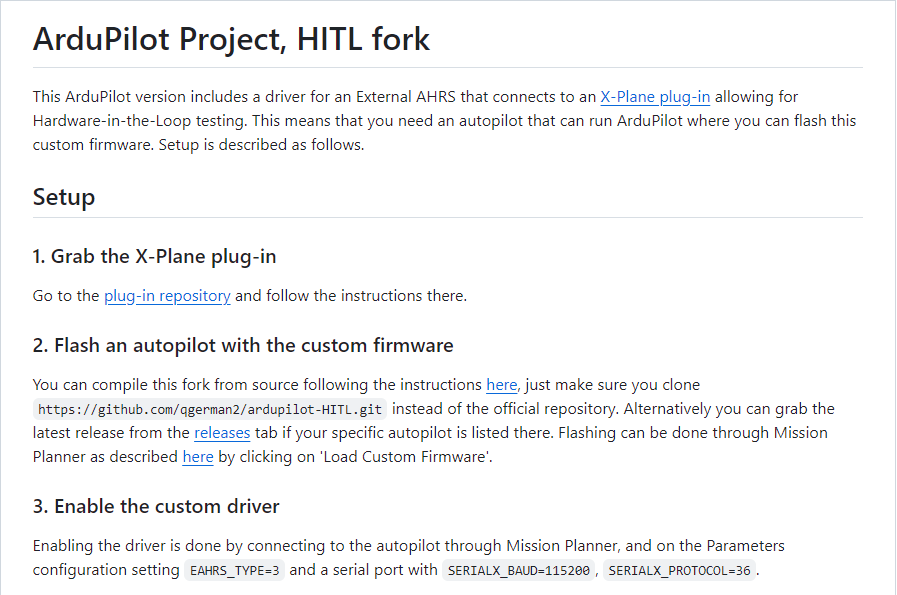
\includegraphics[width=0.7\textwidth]{repo-ap.png}
    \caption{Instrucciones en repositorio de fork de ArduPilot.}
    \label{fig:repo-ap}
\end{figure}

\begin{figure}[h]
    \centering
    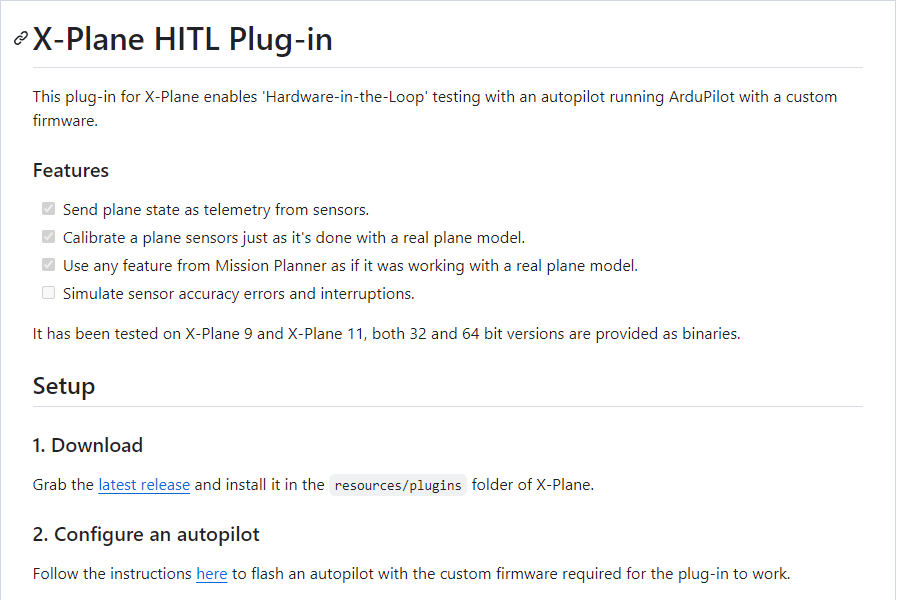
\includegraphics[width=0.7\textwidth]{repo-plugin.png}
    \caption{Instrucciones en repositorio de plug-in para X-Plane.}
    \label{fig:repo-plugin}
\end{figure}